\documentclass[a5paper,headsepline,titlepage,11pt,nnormalheadings,DIVcalc]{scrbook}
\usepackage[a5paper,backref]{hyperref}
\usepackage[papersize={148.5mm,215mm},twoside,bindingoffset=0.5cm,hmargin={2cm,2cm},
				vmargin={2cm,2cm},footskip=1.1cm,driver=dvipdfm]{geometry}
%\usepackage{palatino}
\usepackage{graphicx}
\usepackage{wrapfig}
\usepackage[bahasa]{babel}
\usepackage{fancyhdr}
\usepackage{longtable}
\usepackage{hhline,multirow}
\usepackage{pst-node}

%\setlength{\voffset}{0.5in}
%\setlength{\oddsidemargin}{28pt}
%\setlength{\evensidemargin}{0pt}
\renewcommand{\footrulewidth}{0.5pt}
\lhead[\fancyplain{}{\thepage}]%
      {\fancyplain{}{~}}
\rhead[\fancyplain{}{~}]%
      {\fancyplain{}{\thepage}}
\pagestyle{fancy}
\lfoot[\emph{Doa 40 hari \namaalm}]{}
\rfoot[]{\emph{Lingkungan St Petrus Maguwo}}
\cfoot{}

\newcommand{\BU}[1]{\begin{itemize} \item[U:] #1 \end{itemize}}
\newcommand{\BI}[1]{\begin{itemize} \item[I:] #1 \end{itemize}}
\newcommand{\BP}[1]{\begin{itemize} \item[P:] #1 \end{itemize}}
\newcommand{\BPP}[1]{\begin{itemize} \item[Bpk:] #1 \end{itemize}}
\newcommand{\BPW}[1]{\begin{itemize} \item[Ibu:] #1 \end{itemize}}
\newcommand{\namaalm}{Ibu MG Ari Tri Wuryanti~}
\newcommand{\namaromo}{~}
\title{Ibadat/Doa untuk Arwah}
\author{}
\date{2010}
\hyphenation{sa-u-da-ra-ku}
\hyphenation{ke-ri-ngat}
\hyphenation{je-ri-tan}
\hyphenation{hu-bung-an}
\hyphenation{me-nya-dari}
\hyphenation{Eng-kau}
\hyphenation{ke-sa-lah-an}
\hyphenation{ba-gai-ma-na}
\hyphenation{Tu-han}
\hyphenation{di-per-ca-ya-kan}
\hyphenation{men-ja-uh-kan}
\hyphenation{bu-kan-lah}
\hyphenation{per-sa-tu-kan-lah}
\hyphenation{ma-khluk}
\hyphenation{Sem-buh-kan-lah}
\hyphenation{ja-lan}
\hyphenation{mem-bu-tuh-kan}
\hyphenation{be-ri-kan-lah}
\hyphenation{me-ra-sa-kan}
\hyphenation{te-man-ilah}
\hyphenation{mem-bi-ngung-kan}
\hyphenation{di-ka-gum-i}
\hyphenation{ta-ngis-an-Mu}
\hyphenation{mi-lik-ilah}

\renewcommand*\thesection{\arabic{section}.}
\setlength{\parindent}{0mm} 

\begin{document}
\thispagestyle{empty}
%\maketitle
%\newsavebox\IBox
%\sbox\IBox{\includegraphics[scale=0.4]{Saint-Peter-Apostle-e.eps}}

\psset{unit=1in}
\begin{pspicture}(4in,6.0in)
% set up the fonts we use
\DeclareFixedFont{\PT}{T1}{ppl}{b}{it}{0.4in}
\DeclareFixedFont{\PTsmall}{T1}{ppl}{b}{it}{0.3in}
\DeclareFixedFont{\PTsmallest}{T1}{ppl}{b}{it}{0.2in}
\DeclareFixedFont{\PTtext}{T1}{ppl}{b}{it}{11pt}
\DeclareFixedFont{\Logo}{T1}{pbk}{m}{n}{0.2in}
% place the front cover picture
%\rput[cb](2.3,2.5){\usebox\IBox}
% put the text on the front cover
\rput[cb](2.5,5.3){\PTsmall {Ibadat/Doa Arwah 40 hari untuk}}
\rput[cb](2.5,4.8){\PTsmall {\namaalm}}
\rput[cb](2.5,1.1){\PTsmall {10 April 2010}}
\rput[cb](2.5,0.6){\PTsmallest {Wilayah Yohanes de Britto}}
\rput[cb](2.5,0.3){\PTsmallest {Stasi Maguwo}}
\rput[cb](2.5,0.0){\PTsmallest {Paroki Marganingsih Kalasan }}

%\rput[cb](3,-1){\PTsmallest {\namagereja}} 

\end{pspicture}
%\tableofcontents 
\newpage
\thispagestyle{empty}
{~}
\newpage
\setlength{\parskip}{2mm}

\section*{RITUS PEMBUKA}
\subsection*{LAGU PEMBUKA}

\subsection*{SALAM PEMBUKAAN}
\BP{Atas nama Bapa Putera dan Roh Kudus} 
\BU{Amin}
\BP{Semoga damai sejahtera Tuhan kita Yesus Kristus, cinta kasih Allah Bapa dan persekutuan Roh Kudus, selalu beserta kita.}
\BU{Sekarang dan selama-lamanya}

\subsection*{PENGANTAR}
\BP{Bapak Ibu Saudara Saudari Anak-anak yang terkasih dalam Kristus, 40 hari yang lalu keluarga ini mengalami duka yang mendalam. Kalau ditanya mengapa berduka? Jawabanya adalah karena pada waktu itu \namaalm telah dipanggil Tuhan. Mungkin kita bisa ikut merasakan perasaan / suasana hati dari keluaraga yang ditinggalkan pada waktu itu. Sebagai ungkapan cinta keluarga ini terhadap almarhumah \namaalm kita semua diundang untuk bersama-sama mendukung dengan doa-doa supaya arwah dari \namaalm segera dapat ikut bangkit mulia bersama Kristus di dalam kerajaan surga.}

\emph{Hening sejenak \dots}
  
\subsection*{PERNYATAAN TOBAT}
\BP{Saudara-saudari yang seiman dalam Kristus, marilah kita membuat diri pantas berada di depan hadirat Allah, dengan membersihkan diri kita dari dosa dan kesalahan yang lalu, dengan bertobat dan mohon ampun kepada Allah kita.}

\BP{Saya mengaku \dots}

\BP{Semoga Allah yang mahakuasa mengasihani kita, 
mengampuni dosa kita dan mengantar kita ke dalam hidup 
yang kekal.}

\BU{Amin}

\subsection*{Doa Pembuka}
\BP{Marilah Berdoa 

Allah Bapa yang mahamurah, Engkau telah menyerahkan 
Yesus, Putra-Mu kepada kematian, semua ini harus terjadi 
untuk melepaskan kami dari segala kuasa kegelapan dan 
dosa. Ya Bapa, anugerahkanlah hidup kekal kepada 
saudara-saudari ……….yang telah menghadap 
kehadiratMu 40 hari yang lalu. Ya Bapa, ampunilah 
segala dosa dan kesalahannya dan bukalah pintu 
kehidupan kekal baginya. Terimalah saudara kami 
tercinta ini kedalam keluarga kudusMu di tahta surgawi. }

\BU{Amin} 
 
\section*{IBADAT SABDA}
\BP{Saudara-saudari terkasih marilah kita mempersiapkan hati 
dan budi untuk mendengarkan sabda Tuhan.} 

\subsection*{BACAAN PERTAMA}

\BP{Pembacaan dari Kitab Nabi Yesaya (25: 7-9) 

Dan diatas gunung ini Tuhan akan mengoyakkan kain 
perkabungan yang diselubungkan kepada segala suku bangsa 
dan tudung yang ditudungkan kepada segala bangsa-bangsa. Ia 
akan meniadakan maut untuk seterusnya ; dan Tuhan Allah 
akan menghapuskan air mata dari pada segala muka ; dan aib 
umatNya akan dijauhkanNya dan seluruh bumi, sebab Tuhan 
telah mengatakannya. Pada waktu itu orang akan berkata : 
“Sesungguhnya, inilah Allah kita, yang kita nanti-nantikan, 
supaya kita diselamatkan. Inilah Tuhan yang kita nantinantikan 
; marilah kita bersorak-sorak dan bersukacita oleh 
karena keselamatan yang diadakan-Nya !” 

Demikianlah sabda Tuhan }

\BU{Syukur kepada Allah} 

\subsection*{Antar Bacaan} 

\subsection*{Bacaan Injil} 

\BP{Tuhan sertamu} 
\BU{Dan sertamu juga} 
\BP{Inilah Injil Yesus Kristus menurut Yohanes (6:37-47) 

Semua yang diberikan Bapa kepada-Ku akan datang kepada-Ku, dan barangsiapa datang kepada-Ku, ia tidak akan Kubuang.
Sebab Aku telah turun dari sorga bukan untuk melakukan kehendak-Ku, tetapi untuk melakukan kehendak Dia yang telah mengutus Aku.

Dan Inilah kehendak Dia yang telah mengutus Aku, yaitu supaya dari semua yang telah diberikan-Nya kepada-Ku jangan ada yang hilang, tetapi supaya Kubangkitkan pada akhir zaman.
Sebab inilah kehendak Bapa-Ku, yaitu supaya setiap orang, yang melihat Anak dan yang percaya kepada-Nya beroleh hidup yang kekal, dan supaya Aku membangkitkannya pada akhir zaman."

Maka bersungut-sungutlah orang Yahudi tentang Dia, karena Ia telah mengatakan: "Akulah roti yang telah turun dari sorga."

Kata mereka: "Bukankah Ia ini Yesus, anak Yusuf, yang ibu bapanya kita kenal? Bagaimana Ia dapat berkata: Aku telah turun dari sorga?"

Jawab Yesus kepada mereka: "Jangan kamu bersungut-sungut.
Tidak ada seorangpun yang dapat datang kepada-Ku, jikalau ia tidak ditarik oleh Bapa yang mengutus Aku, dan ia akan Kubangkitkan pada akhir zaman.

Ada tertulis dalam kitab nabi-nabi: Dan mereka semua akan diajar oleh Allah. Dan setiap orang, yang telah mendengar dan menerima pengajaran dari Bapa, datang kepada-Ku.
Hal itu tidak berarti, bahwa ada orang yang telah melihat Bapa. Hanya Dia yang datang dari Allah, Dialah yang telah melihat Bapa.

Aku berkata kepadamu: Sesungguhnya barangsiapa percaya, ia mempunyai hidup yang kekal.

Demikianlah Injil Tuhan} 

\BU{Terpujilah Kristus}

\subsection*{HOMILI}

Bapak Ibu Sdr/Sdri yang baik sosok ibu adalah seseorang yang bagi kebanyakan orang sebagai orang yang paling dekat dengan kita. Bagaimana tidak coba kalau kita amati bayi, kata ibu/mama itu adalah kata pertama yang dapat diucapkan oleh seorang bayi, seperti anak saya……. baru setelah beberapa Minggu yang mulai menyebut nama Bapak. Sesudah agak besar sekita 5 tahun kalau sedang asik bermain lari-lari tiba-tiba jatuh dan menangis maka kata kata Ibu / Mama lah yang disebut. Bagi kita yang sudah cukup umur kalau mengalami kesulitan / mengalami musibah kita acap kali juga menyebut nama ibu. Dari semua contoh tersebut saya mau mengatakan betapa berartinya, betapa dekatnya kita dengan seorang ibu.

Saudara kita keluarga ini belum lama juga ditinggal orang yang sangat dekat juga yang sangat dicintai dan mestinya peristiwa itu belum sepenuhnya dapat dilupakan begitu saja. \namaalm sewaktu hidupnya telah mengikuti Kristus dan menjadi muridnya yang setia. Ini telah dibuktikanya dalam kesetiaanya memanggul salib kehidupanya dan mempertahankan Imannya sampai Kristus memanggilnya kembali. Dalam bacaan tadi Tuhan berfirman “ Aku berkata kepadamu: Barang siapa percaya kepada-Ku, ia mempunyai hidup yang kekal. Kiranya Almarhumah \namaalm diberikan kehidupan yang kekal karena ia juga mengimani Kristus semasa hidupnya.

Bapak Ibu Saudara Saudari yang terkasih dibagian yang lain injil malam ini juga menyebutkan sebagai berikut “ Dan inilah kehendak Bapa, Dia yang telah mengutus Aku, yaitu supaya dari semua yang telah diberikan-Nya kepada-Ku jangan ada yang hilang, tetapi supaya Aku membangkitkanya pada akhir jaman. Kemudian kalau kita lihat hidup dari \namaalm telah meyerahkan tidak hanya dirinya sendiri, tetapi juga seluruh keluarganya dan putra putrinya menjadi pengikut Kristiani yang mengandalkan Yesus Kristus sebagai satu-satunya penyelamat. Tentunya \namaalm juga akan dibangkitkan kembali bersama Kristus.

Bapak Ibu Sdr sekalian berdasarkan iman kepercayaan kita , sekarang menjadi jelas bahwa kepergian \namaalm bukanlah kefanaan, bukan pula suatu kebinasaan melainkan suatu awal untuk bersatu dengan Kristus, bangkit dan mulia di dalam kerajaan-Nya. Amin
Marilah kita lanjutkan dengan doa umat

\section*{DOA}

\subsection*{DOA UMAT}

\BP{Allah Bapa kami yang maha kasih dan penyayang, kami menghadap hadiratmu untuk menyampaikan ungkapan hati dan permohonan kami. Kami percaya Engkau akan selalu berkenan menyertai kami, mendengarkan kami dan memberikan yang terbaik bagi kami. Kami memuji dan memuliakan nama-Mu melalui doa-doa ini:}

\BP{Ya Tuhan Yesus Kristus penyelamat dunia kami mempercayakan kepadamu arwah \namaalm, berkenanlah engkau menerimanya dalam sukacita kerajaan-Mu

Kami mohon}

\BU{Kabulkanlah doa kami ya Tuhan}

\BP{Ya Allah, kami mohon kemurahaanmu bagi \namaalm , janganlah kau ingat-ingat lagi dosa-dosanya, tetapi limpahkanlah kerahiman-Mu kepadanya. Semoga Ia disambut dan dipersatukan bersama para malaikat dan orang kudus di surga.

Kami mohon}

\BU{Kabulkanlah doa kami ya Tuhan}

\BP{Bagi keluarga yang ditinggalkan, ya Bapa tolonglah mereka semua supaya saling mendukung , saling memberi kekuatan dan penghiburan. Semoga kenangan akan masa hidup \namaalm akan tersimpan dalam hati mereka, dan meneguhhkan kepercayaan mereka akan bimbingan-Mu 

Kami mohon}

\BU{Kabulkanlah Doa kami ya Tuhan} 

\BP{Ya Bapa Keluarga ini telah menyerahkan seluruh hidupnya kedalam penyelenggaraan-Mu, maka sudilah mendampingi mereka supaya sanggup menghadapi liku-liku hidup ini , lebih-lebih saat ini dikala keluarga ini ditinggalkan oleh ibu yang mereka cintai.

Kami mohon}

\BU{Kabulkanlah doa kami ya Tuhan}

\BP{Bagi kita semua yang berhimpun disini beserta keluarganya, ya Bapa jadikanlah kami alat-Mu dalam menciptakan kerukunan dan penghiburan dan pembawa damai. Jauhkanlah kami semua dari kemalangan.

Kami mohon}

\BU{Kabulkanlah doa kami ya Tuhan}

\BP{Demikianlah ya Bapa, doa-doa yang kami panjatkan. Engkau mengetahui keinginan keinginan dan kesulitan kami. Kami percaya akan penyelenggaraan-Mu dan bersama Roh Kudus, kami senantiasa belajar utuk memahami apa yang sebenarnya Engkau kehendaki atas diri kami . Kami menyampaikan doa-doa kami ini dengan perantaraan Putera-Mu terkasih, Tuhan kami Yesus Kristus, yang hidup dan berkuasa kini dan sepanjang masa. Amin}


\subsection*{DOA BAPA KAMI}
Marilah kita satukan doa-doa permohonan kita dengan doa yang diajarkan Yesus sendiri 
Bapa kami yang ada di surga \dots .( didoakan bersama sama )

\subsection*{ROSARIO}
Bapak Ibu Saudara Saudari, Ibu Maria telah memberikan teladan bagi kita. Ia telah setia mendampingi Puteranya Tuhan Yesus Kristus sampai wafatnya di kayu salib. Marilah kita mohon lewat perantaraan Bunda maria supaya mendampingi arwah \namaalm dalam mengahapap Bapa dengan doa Rosario.

Aku percaya

Bapa kami…….

Kemuliaan kepada Bapa ……

Terpujilah ……

Salam Putri Allah Bapa. Salam Maria……

Salam Bunda Allah Putera. Salam Maria….

Salam Mempelai Allah Roh Kudus. Salam Maria …..  

Kemuliaan…

Terpujilah…

Ya Bapa terimah arwah \namaalm dalam kemuliaan kerajaan-Mu.

\section*{RITUS PENUTUP}

\subsection*{DOA PENUTUP}
\BP{Marilah berdoa :
 
Allah Bapa kami yang mahapengasih dan penyanyang, 
semoga kebangkitan putraMu juga menjadi kebangkitan 
saudara kami \namaalm  Bapa semoga Engkau senantiasa 
membangkitkan semangat kami untuk terus menerus hidup 
seturut nasihat InjilMu. Bapa, semoga doa-doa yang kami 
panjatkan kehadiratMu mampu mengantar saudara-saudari 
kami yang sudah meninggal untuk memasuki kerajaanMu 
yang abadi di surga. }
\BU{Amin} 

\subsection*{BERKAT}
\BP{Tuhan beserta kita}
\BU{Sekarang dan selama-lamanya}
\BP{Semoga kita semua, keluarga kita dan karya kita selalu di bimbing dan diberkati oleh Bapa dan Putera dan Roh Kudus.}

\BU{Amin}

\BP{Saudara sekalian ibadat kita sudah selesai marilah kita mundur dalam damai Tuhan}
\BU{Syukur kepada Allah.}

\subsection*{LAGU PENUTUP}

\end{document}